\documentclass[conference]{IEEEtran}
\PassOptionsToPackage{table}{xcolor}
\IEEEoverridecommandlockouts

% The preceding line is only needed to identify funding in the first footnote. If that is unneeded, please comment it out.
\renewcommand\IEEEkeywordsname{Keywords}

\usepackage[noadjust]{cite}
\renewcommand{\citepunct}{,\penalty\citepunctpenalty\,}
\renewcommand{\citedash}{--}
\usepackage{caption}
\usepackage{url}
\usepackage{titletoc}
\usepackage{amsmath,amssymb,amsfonts}
\usepackage{algorithmic}
\usepackage{graphicx}
\usepackage{textcomp}
\usepackage{bm}
\usepackage{booktabs}
\usepackage{multirow}
\usepackage{tikz}
\usepackage{pgfplots}
\def\BibTeX{{\rm B\kern-.05em{\sc i\kern-.025em b}\kern-.08em
    T\kern-.1667em\lower.7ex\hbox{E}\kern-.125emX}}
\pgfplotsset{compat=1.14}

\newcommand{\Rplus}{\protect\hspace{-.1em}\protect\raisebox{.35ex}{\smaller{\smaller\textbf{+}}}}
\newcommand{\Cpp}{\mbox{C\Rplus\Rplus}\xspace}
\usepackage[utf8]{inputenc}
\usepackage{listings}
\usepackage[T1]{fontenc}
\usepackage{xcolor}
\usepackage{algorithm}
\usepackage{algorithmic,eqparbox,array}
\captionsetup[listing]{font={stretch=1.2}}

\definecolor{lightgray}{rgb}{.9,.9,.9}
\definecolor{darkgray}{rgb}{.4,.4,.4}
\definecolor{purple}{rgb}{0.65, 0.12, 0.82}

% auto labeling of sections
\let\origsection=\section
\renewcommand\section[1]{\origsection{#1}\label{sec:{#1}}}

\let\origsubsection=\subsection
\renewcommand\subsection[1]{\origsubsection{#1}\label{subsec:{#1}}}

\let\origsubsubsection=\subsubsection
\renewcommand\subsubsection[1]{\origsubsubsection{#1}\label{subsubsec:{#1}}}

\lstdefinelanguage{JavaScript}{
  keywords={typeof, new, false, catch, function, return, null, catch, switch, var, if, in, while, do, else, case, break},
%   keywordstyle=\color{blue}\bfseries,
  ndkeywords={class, export, boolean, throw, implements, import, this, type, interface, extends},
%   ndkeywordstyle=\color{darkgray}\bfseries,
%   identifierstyle=\color{black},
  sensitive=false,
  comment=[l]{//},
  morecomment=[s]{/*}{*/},
%   commentstyle=\color{purple}\ttfamily,
%   stringstyle=\color{red}\ttfamily,
  morestring=[b]',
  morestring=[b]"
}

% \lstset{
%   language=JavaScript,
% %   backgroundcolor=\color{lightgray},
% %   columns=fullflexible,
%   extendedchars=true,
%   basicstyle=\footnotesize\ttfamily,
%   showstringspaces=false,
%   showspaces=false,
% %   numbers=left,
%   numberstyle=\footnotesize,
%   numbersep=9pt,
%   tabsize=2,
%   breaklines=true,
%   showtabs=false,
%   captionpos=b
% }

\def\thesubsubsectiondis{\unskip\arabic{subsubsection})}

\renewcommand{\ttdefault}{pcr}
\lstset{
    aboveskip=0.2cm,
    stringstyle=\ttfamily,
    showstringspaces = false,
    basicstyle=\scriptsize\ttfamily,
    commentstyle=\color{gray!85},
    keywordstyle=\bfseries,
    ndkeywordstyle=\bfseries,
    identifierstyle=\ttfamily,
    numbers=none,
    % numbersep=5pt,
    % numberstyle=\tiny,
    % numberfirstline = false,
    breaklines=true,
    tabsize=2,
    % frame=L,
    rulecolor=\color{black},
    captionpos=t,
    % escapeinside=##
    breakatwhitespace=true,
    belowcaptionskip=10pt
    % xleftmargin=10pt
}

% \lstset{
%   basicstyle=\ttfamily,
%   columns=fullflexible,
%   frame=single,
%   breaklines=true,
%   basicstyle=\footnotesize, %or \tiny or \small etc.
% %   postbreak=\mbox{\textcolor{red}{$\hookrightarrow$}\space},
% }

\usepackage{hyperref}


\hypersetup{
    colorlinks=true,
    linkcolor=blue,
    filecolor=magenta,      
    urlcolor=brown,
    pdfpagemode=FullScreen,
    }
    
\usepackage{multicol}


\usepackage{tabulary}

\definecolor{Mycolor1}{HTML}{4C5866} %#4C5866
\definecolor{Mycolor2}{HTML}{A6B6D2} %#A6B6D2
\definecolor{Mycolor3}{HTML}{C1D4E8} %#C1D4E8
\definecolor{Mycolor4}{HTML}{F7F7FE} %#F7F7FE
\definecolor{Mycolor5}{HTML}{d8f3dc} %#d8f3dc
\definecolor{Mycolor6}{HTML}{EC6A5C} %#EC6A5C
\definecolor{Mycolor7}{HTML}{EDE992} %#EDE992


% Switch for algorithmic
\newcommand{\Switch}[1]{\STATE \textbf{switch} (#1)}
\newcommand{\EndSwitch}{\STATE \textbf{end switch}}
\newcommand{\Case}[1]{\STATE \textbf{case} #1\textbf{:} \begin{ALC@g}}
\newcommand{\EndCase}{\end{ALC@g}}
\newcommand{\Caseline}[1]{\STATE \textbf{case} #1\textbf{:} }
\newcommand{\Default}{\STATE \textbf{default:} \begin{ALC@g}}
\newcommand{\EndDefault}{\end{ALC@g}}
\newcommand{\DefaultLine}[1]{\STATE \textbf{default:} }
\newcommand{\edit}[2]{\textcolor{blue}{#1} \textcolor{red}{#2}}
\newcommand{\atlas}[1]{\textcolor{brown}{#1}}
\newcommand{\atlass}[2]{\textcolor{brown}{#1} \textcolor{pink}{original: #2}}


\newcommand{\red}[1]{\textcolor{red}{#1}}
\newcommand{\doubt}[1]{\textcolor{purple}{#1}}

\begin{document}

\title{RSS3: A Next-Generation Feed Standard}

%\titlerunning{Abbreviated paper title}
% If the paper title is too long for the running head, you can set
% an abbreviated paper title here
%
\author{Natural Selection Labs}
\maketitle              % typeset the header of the contribution

\thispagestyle{plain}
\pagestyle{plain}
\pagenumbering{arabic}

\begin{abstract}

Inspired by the original RSS Standard, this paper presents RSS3, the next-generation feed standard, that aims to support efficient and decentralized information distribution. Furthermore, the RSS3 Protocol is proposed in conjunction with a sophisticated network structure to implement the standard. The result is a fully decentralized network that is flexible, efficient, and extensible.

\end{abstract}

\section{Introduction}

RSS3 is the \glsfmtlong{OIL}, structuring \glsfmtlong{OI} for social, search, and AI.
The \gls{OIL} is a decentralized and permissionless layer where information flows openly without any restrictions, as it is supposed to be.

It is RSS3's mission to construct the \glsfmtlong{OW} by enhancing the free flow of \glsfmtlong{OI}.



\section{glossary}

This section includes the glossary Table~\ref{table:glossary} contains a list of terms used throughout the paper.

{
\renewcommand{\arraystretch}{1.5}
\begin{table}[!ht]
	\rowcolors{2}{}{Mycolor1!10}
    \resizebox{\columnwidth}{!}{
		\begin{tabulary}{\columnwidth}{|l|p{8cm}|}
			\hline
			\rowcolor{Mycolor1!30} \multicolumn{1}{|l|}{\textbf{Term}}&\multicolumn{1}{|l|}{\textbf{Definition}}\\
			\hline
			% \atlas{Shark} & A Shark refers to a collection of data generated by one cyber existence.\\
			% \hline
    		DAO & Decentralized Autonomous Organization, an automated decision-making organization that is agreed by the network and is not influenced by a central authority. DAO oversees all important decisions. \\
    		\hline
    		SN & A serving node, which hosts RSS3 Files and responds to file-related requests. DAO sets a limit of files that a single SN can serve.  \\
    		\hline
    		Subgroup & A group of SNs, which consists of a number of SNs. DAO sets a limit of SNs that a single subgroup can have.  \\
    		\hline
    		GI & A global indexer, which orchestrates subgroups, routes client requests, and maintains the network capability. DAO sets the incentive scheme. \\
    		\hline
    		RN & A relay node, as part of a GI to assist in routing. \\
    		\hline
    		Epoch & A reference point in time where multiple events are scheduled to be triggered. \\
    		\hline
    		ER & Epoch round, a period of time between two epoch points where the network operates without any planned events from DAO and GIs. DAO sets the ER interval. \\
    		\hline
    		SDG & Scalable Dynamic Grouping, the strategy used by GIs to orchestrate subgroups that will be executed at the epoch.  \\
			\hline
			MOC & Minimal operational capability, the required number of GIs or SNs in a subgroup, to provide trustworthy services. \\
			\hline
			HBC & Heartbeat checking, a strategy used by nodes to report their working status. \\
			\hline
		\end{tabulary}
		
	}
	\caption{A glossary table that contains the terms used throughout the paper.}
	\label{table:glossary}
\end{table}
}

\section{Standard} 

% put the figure here for formatting reasons
\begin{figure*}[tb!]
    \centering
    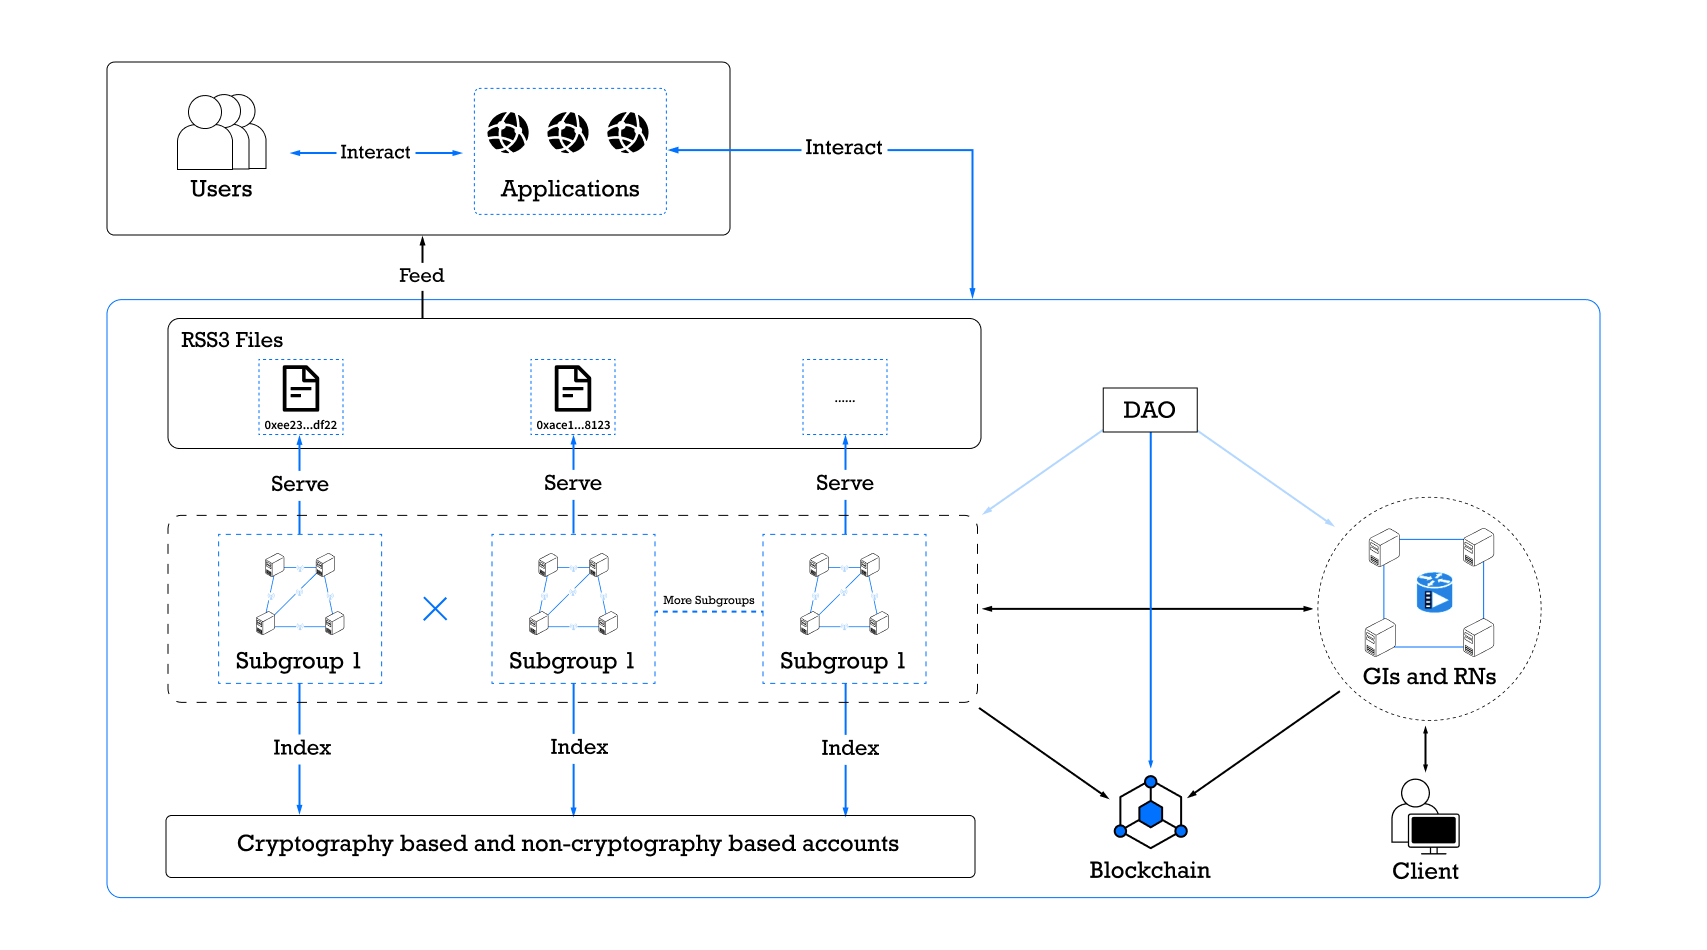
\includegraphics[height=9.3cm]{figures/network-arch.jpg}
    \caption{A typical RSS3 Network architecture.}
    \label{fig:network-arch}
\end{figure*}

Compared to its predecessor, RSS3 introduces fundamental changes to create an efficient and decentralized information distribution standard.

\subsection{Instance}

An instance is a collection of cryptography based accounts owned by one cyber existence. Upon registration, the first address submitted will be used as the instance's primary address. Additional accounts can be imported by auto-verification or user actions. All verified accounts will be stored in an RSS3 File. 

\subsection{Asset}

An asset refers to a medium of exchange owned by the instance that is digitally generated. An RSS3 network automatically incorporates instance assets from verified accounts, and stores them into the corresponding RSS3 File. DAO decides the rendering of assets in RSS3 Files as there are wide variations in types.

\subsection{Link}

Ubiquitous linking is the foundation of an open information system. The RSS3 Protocol supports universal links with customized types between RSS3 Objects. Major RSS3 Objects include:

\begin{itemize}
    \item Instance - a collection of cryptography based accounts
    \item Asset - a medium of exchange that is digitally generated
    \item Item - content generated on the network
\end{itemize}

An internal link is bidirectional which connects two objects within an RSS3 Network, whereas an external link unidirectionally connects an RSS3 Object with an external object. An external link destined for an RSS3 Object may be bidirectional if DAO approves the source.

\subsection{Governance and Ownership}

RSS3 network is equipped with a high Turing completeness. It is capable of handling sophisticated logic such as reviewing smart contracts that define permission and ownership of RSS3 Files.

\subsection{Activity Feed}

In an RSS3 File, an activity feed contains: 1) all activities indexed from the instance's verified accounts; 2) all items generated by the instance or the network; 3) all universal links generated on the RSS3 Network. The feed resembles the original RSS protocol with additional cryptographic information to support data integrity and originality. The design represents a decentralized approach for information distribution.

Based on the standard described above, we present the RSS3 Protocol, available at \url{https://github.com/NaturalSelectionLabs/RSS3}. The implementation is by no means a perfect solution to the problems which the web is facing now, but a significant leap forward toward a truly decentralized cyberspace.


\section{\glsfmtlong{R3N}}

The \glsfmtlong{R3N} is a decentralized network that is formed by two Sublayers: the \glsfirst{DSL} and the \glsfirst{VSL}.
This novel network structure is the product of a series of research and development experiments, that were conducted to address the challenges faced by the Open Web.

\gls{OI} is typically found across various types of networks, including decentralized, federated, and centralized networks that allow permissionless access.
The \gls{DSL} is responsible for indexing and structuring \gls{OI} for interoperability.
This is achieved by introducing a crucial standard, known as the \gls{UMS}, see \Cref{subsec:UMS}, enabling network-agnostic applications to be built on top of the \gls{DSL}.
The \gls{DSL} then leverages the \gls{VSL}, see \Cref{sec:VSL}, to build an ownership economy for the \gls{OW}.

\subsection{\$RSS3}
\$RSS3 is the Network's native utility token. It is used to cover gas, pay request fees, operate nodes, participate in staking and trust, distribute incentives, and engage in various network activities. See \Cref{sec:tokenomics} for more details.

\subsection{\Glsfmtfull{Epoch}}

An \glsfirst{Epoch} is a period of time used as a reference to measure the RSS3 Network’s operation, during which the Network's parameters are fixed.
The duration of an epoch is determined by the Network, and is subject to potential future changes.

At the end of each \epoch, the Network will distribute the \gls{NR} to the \glsfmtlong{R3N}'s participants, and update the Network's parameters when necessary.

\section{Incentive}

\subsection{Incentivization}

The RSS3 Network, on the other hand, will be rewarding network participants with the profit of the network generated from advertising, value-added services, social economic activities, etc.

\subsection{Staking and Slashing}

\subsection{Incentive Pool}

\subsubsection{Operator Pool}

\subsubsection{Reward Pool}


\section{Scalability}


\section{Vulnerability}

\subsection{Collusion}
In an RSS3 Network, RSS3 Files are hosted by subgroups of SNs for redundancy and fault tolerance. Although the subgroup design creates the bedrock for potential collusive behaviors, the design itself also acts as the first layer to prevent those behaviors since an internal consensus is required to process all client requests. A client request, as illustrated in Fig.~\ref{fig:network-arch}, is forwarded from GIs to SNs and returned back to GIs consequently. GIs then return the most consistent result back to the client. Furthermore, a collusion will not have any impact on the result when the number of malicious or erroneous nodes, denoted $\mathcal{M}$, where $\mathcal{M} \le \mathcal{P}$.

The probability of a collusion taking place, though slim, still exists in theory. GIs minimize this probability through breaking potential $\mathcal{M}$ via SDG, as described in Sec.~\ref{subsubsec:{Scalable Dynamic Grouping (SDG)}}. SNs within the same subgroup are less likely to be grouped together in the future to prevent possible collusion.

Unlike blockchain-based networks, the collusion in the RSS3 Network is not economically profitable, which eliminates the primary motivation behind collusion\cite{schrepel2019Collusion}. In the event of a collusion, owners can correct tampered data at any time and report SNs for malicious behaviors. Collusive SNs lose their incentives and seats in the network. Since staking is required, slashing also serves as a deterrent to potential colluders.

\subsection{Redundancy}
Subgrouping provides redundancy as SNs: 1) maintain RSS3 Files assigned collaboratively, effectively creating $\mathcal{S}$ copies for redundancy; 2) are with best efforts distributed across the globe to provide geo-redundancy and sustain a high availability.

During the election, DAO selects GIs from multiple regions to provide geo-redundancy.

\subsection{Disaster Recovery}

To recover from an unlikely event of a complete network failure, where more than $\mathcal{R}_g$ GIs or $\mathcal{R}_{s}$ SNs have failed to stay functional, see Eqn.~\ref{disaster-recovery}, DAO members may operate archive modules that constantly take snapshots of the entire network. GIs are also encouraged to operate archive modules.

\begin{equation}
\mathcal{R}_{(g \lor s)} = \lfloor\frac{\mathcal{(G \lor S)}}{3}\rfloor; \forall \mathcal{(G \lor S)} \in \mathbb{N}^+
\label{disaster-recovery}
\end{equation}

\subsection{Sybil Attack}
Sybil attacks may occur in any network, where a disproportionate level of network resources are allocated to attackers, affecting the network's availability. Research shows that there is currently no universally applicable solution to Sybil attacks\cite{douceur2002Sybil}. In the RSS3 Network, such an attack does not generate any financial gains. Furthermore, identity validation is implemented to minimize the chance of Sybil attacks. The network also increases the economic costs for such an attack.


\section{Conclusion} 

\textbf{At the heart of Natural Selection Labs, we firmly believe in the freedom of information distribution: No organizations or authorities shall prohibit the free exercise of the right of people to create, store, and distribute their information.}

\let\section=\origsection
\bibliography{bibtex/myRefs}
\bibliographystyle{plain}

\end{document}

